\documentclass[12pt,a4paper]{scrartcl}
\usepackage[utf8]{inputenc}
\usepackage[T1]{fontenc}
\usepackage{lmodern}
\usepackage[ngerman]{babel}
\usepackage{graphicx}
\addtokomafont{disposition}{\rmfamily}

\title{Richtungsanzeiger}
\subtitle{Technischer Entwurf}
\author{Jonas Tochtermann}
\date{\today}
\begin{document}

\maketitle
% \tableofcontents

% \chapter{Kapitel}
\section{Funktionale und nicht-funktionale Anforderungen}

\subsection{Funktionale Anforderungen}

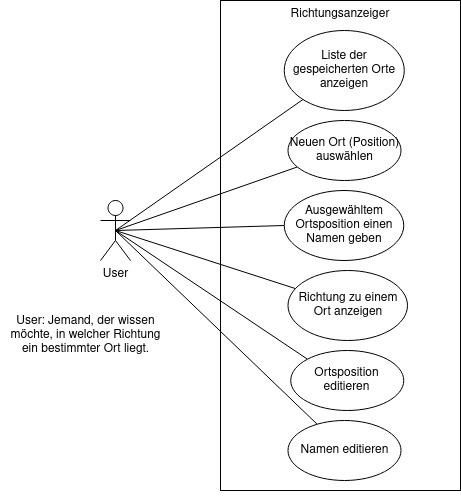
\includegraphics[width=10.0cm]{../UseCase.jpg}

% \subsection{Nicht-funktionale Anforderungen}
%
% \begin{itemize}
%   \item Die Sprache der Benutzeroberfläche ist Deutsch.
%   \item
%   \item
% \end{itemize}
%
% \section{Testkonzept}
%
% \section{Aufbau des Systems}
%
% \section{Visualisierung des Gesamtsystems}

% \subsection{Unterabschnitt}
% \subsubsection{Unterunterabschnitt}
% \paragraph{Paragraph}
% \subparagraph{Unterparagraph}
%
% Hier nun steht schliesslich das Geschriebene.
%
% \dq(Anführungszeichen),~(Leerzeichen ohne Zeilenumbruch),\ (Leerzeichen nicht verbreiterbar),\r {o}, \=o, \'o, \u o, \b o, \d o, \c o, \k o, \`o, \H o, \.o, \~o, \"o, \v o, \t oo, \textcircled o; \AE, \ae, \OE, \oe, \'\AE, \'\ae, \'\OE, \'\oe; äöü ÄÖÜ. ,,a''. -- \textbackslash, \%, \$, \^, \_, \{, \}, \#, \&, \textasciitilde. \i, \j, \dots, \dag, \ddag, Fussnote\footnote{eine Fussnote.}, \emph{Hervorhebung}, hoch\textsuperscript{gestellt}, \textbackslash begin\{quote\} Langzitat \textbackslash end\{quote\}. \texttt{nichtproportional}, \textbf{fett}, \textsc{Kapitälchen}, \textbackslash itemize zur Aufzählung und \textbackslash enumerate zur Nummerierung (mit begin, \textbackslash item und end), ebenso description (items in eckigen Klammern, Doppelpunkt, danach Zeilenumbruch, wahrscheinlich auch Leerzeichen).
%

\end{document}
